\documentclass[a4paper,12pt]{article}

% Packages
\usepackage[utf8]{inputenc}
\usepackage{amsmath}
\usepackage{graphicx}
\usepackage{hyperref}
\usepackage{geometry}
\usepackage{float}

% Page margins
\geometry{left=3cm, right=3cm, top=2cm, bottom=2cm}

% Document settings
\title{Numerical Methods Homework 1}
\author{Nicola Schiavo}
\date{\today}

\begin{document}

\maketitle

\section{Exercise 1}

Consider the initial value problem given by:
\begin{equation}
\begin{cases}
y'(t) = -5y , \\
y(0) = 1.
\end{cases}
\end{equation}
Compute the solution using the 2-step Simpson's method using for the second initial value three different values: the exact solution, estimates with the Runge-Kutta 4 stages methods and with the forward Euler method; consider a stepsize $h = 0.02$ and the final time $T = 6$ .

Simpson formula:  \begin{equation}
    y_{n+2} = y_n + \frac{h}{3} (f_n + 4f_{n+1} + f_{n+2}),
\end{equation}
Forward Euler formula:
\begin{equation}
y_{n+1} = y_n + hf(t_n, y_n)
\end{equation}
Runge Kutta 4-step formula:
\begin{equation}
y_{n+1} = y_n + \frac{1}{6}(k_1 + 2k_2 + 2k_3 + k_4)
\end{equation}
where
\begin{align*}
k_1 &= hf(t_n, y_n), \\
k_2 &= hf\left(t_n + \frac{h}{2}, y_n + \frac{k_1}{2}\right), \\
k_3 &= hf\left(t_n + \frac{h}{2}, y_n + \frac{k_2}{2}\right), \\
k_4 &= hf(t_n + h, y_n + k_3).
\end{align*}

Since the test equation (1) is linear, it's possible to manipulate Simpson's formula (2) and obtain an explicit equation, which will be implemented in the python script:

\begin{equation}
    y_{n+2} =\frac{y_n + \frac{h}{3} (f_n + 4f_{n+1})}{1 + \frac{5}{3}h}
\end{equation}
% Include a figure (Make sure to include the actual file in your LaTeX project)
\begin{figure}[H]
\centering
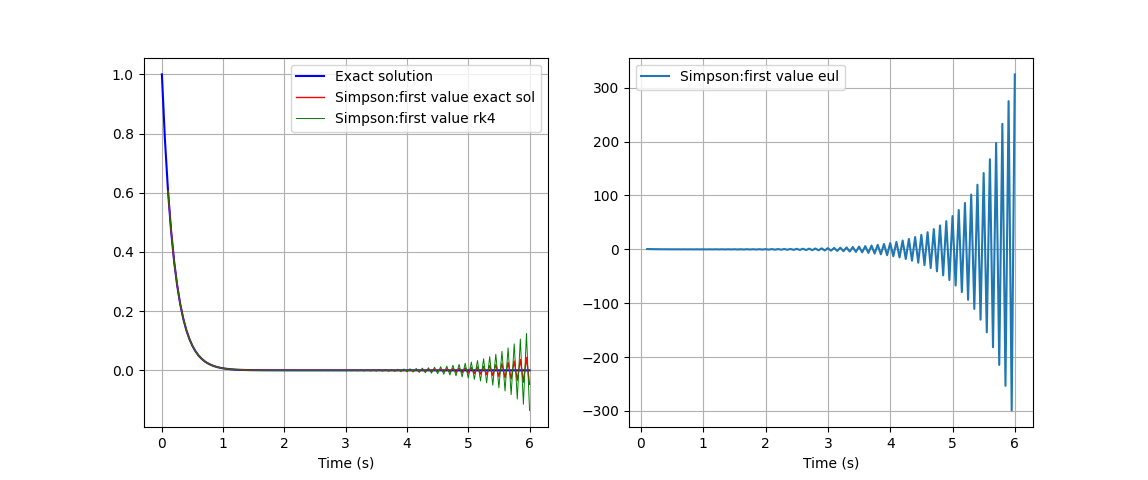
\includegraphics[width=1\textwidth]{simpsons.png}
\caption{The numerical solution obtained by applying the Simpsons method to the test equation.}
\label{fig:simpson_solution}
\end{figure}

\begin{figure}[H]
\centering
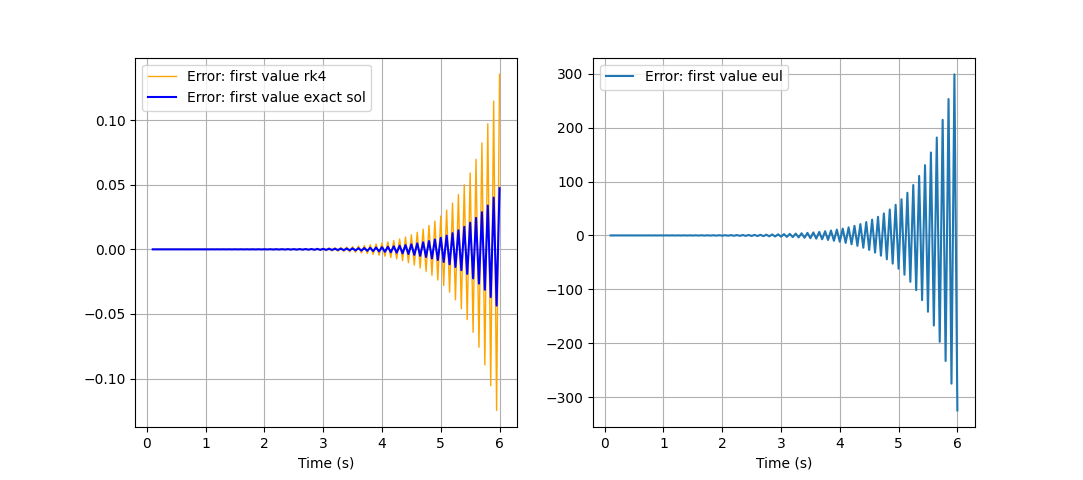
\includegraphics[width=1\textwidth]{simpsons_error.png}
\caption{The error obtained in the three cases.}
\label{fig:simpson_error}
\end{figure}
According to theory, in all cases the method is non stable, as the absolute stability region for Simpson's method is empty.
In fact, I had to make a different figure for the solution computed using forward Euler estimation for the first step, since the error as the difference between estimate and exact solution is three orders of magnitude larger, and it was impossible to appreciate the behaviour of the other cases considered.

\section{Exercise 2}

Consider the initial value problem given by:
\begin{equation}
\begin{cases}
y'(t) = -10y^2 , \\
y(0) = 1.
\end{cases}
\end{equation}
Compute the solution using the 4 stage Runge-Kutta method (4); consider the step sizes $h = 2^{-k}$ for $k = 5,...,10$ , initial time $t_0 = 0$ and final time $T = 2$ .


% Include a figure (Make sure to include the actual file in your LaTeX project)
\begin{figure}[H]
\centering
    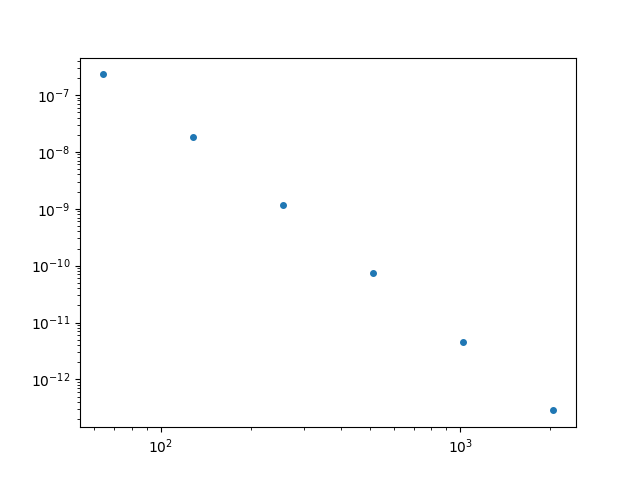
\includegraphics[width=\textwidth]{rk4_error.png} % First image
    \caption{Loglog plot of the error at the final time as a function of the number of steps.}
    \label{fig:rk4_error}
\end{figure}


\begin{tabular}{|c|c|c|}
    \hline
    STEP SIZE & NUMBER OF STEPS & FINAL ERROR \\ \hline
    $2^{-5}$ & 64 & $2.89*10^{-5}$  \\ \hline
    $2^{-6}$ & 128 & $2.03*10^{-6}$  \\ \hline
    $2^{-7}$ & 256 & $8.84*10^{-8}$  \\ \hline
    $2^{-8}$ & 512 & $3.24*10^{-9}$  \\ \hline
    $2^{-9}$ & 1024 & $1.10*10^{-10}$ \\ \hline
    $2^{-10}$ & 2048 & $3.56*10^{-12}$  \\ \hline
    \hline
\end{tabular}
\\[5pt]

Runge-Kutta 4 stages is a method with order of convergence 4, in accordance with the theory , halving the step size the error decrease by roughly a factor 16. 

\section{Exercise 3}

Given two approximations $y_{n+1}^{(h)}$ and $y_{n+2}^{(h/2)}$, which are the solutions at $t_{n+1}$ using step sizes $h$ and $h/2$ respectively, computed with the 4-stages Runge-Kutta method. Assuming that the local truncation error is $C_nh^4$ with $C_n$ depending on the derivatives of $y$, develop a formula for the Richardson extrapolation.

The Richardson Extrapolation formula is:
\begin{equation}
    R(h) = \frac{2^p y(h/2) - y(h)}{2^p - 1}
\end{equation}

For the 4-stage Runge-Kutta method, we assume the error to be $C_nh^4$, hence $p = 4$. Applying this to our approximations, we get:

\begin{equation}
    R(h) = \frac{2^4 y_{n+2}^{(h/2)} - y_{n+1}^{(h)}}{2^4 - 1}
\end{equation}

Simplifying the expression, we obtain:

\begin{equation}
    R(h) = \frac{16 y_{n+2}^{(h/2)} - y_{n+1}^{(h)}}{15}
\end{equation}

This formula provides an extrapolated estimate of the solution at $t_{n+1}$ with a higher order of accuracy than either $y_{n+1}^{(h)}$ or $y_{n+2}^{(h/2)}$ alone.
The error in this extrapolated estimate will be of order $O(h^5)$, assuming the error in the original method is $O(h^4)$.




\section{Exercise 4}
\subsection*{Developing BDF2 formula}
A BDF formula is obtained by first writing the ODE on a point \(t_{n+k}\) as \(y'(t_{n+k}) = f(t_{n+k}, y_{n+k})\). Then the unknown function \(y\) is interpolated at the left hand side of \(y' = f(t, y)\) with a polynomial \(P(t)\) , which will be differentiated.


For \(k = 2\) the interpolator polynomial \(P(t)\) is:

\begin{equation}
P(t) = y_n\frac{(t-t_{n+1})(t-t_{n+2})}{2h^2} + y_{n+1}\frac{(t-t_n)(t-t_{n+2})}{-h^2} + y_{n+2}\frac{(t-t_n)(t-t_{n+1})}{2h^2}
\end{equation}

Computing \(P'(t)\) the terms involving \( (t - t_{n+2}) \) are left out since the polynomial will be evaluated in $t_{n+2}$ and those terms are going to zero.

\begin{equation}
P'(t) = \frac{1}{2h}y_n(t-t_{n+1}) - \frac{1}{h}y_{n+1}(t-t_n) + \frac{1}{2h}y_{n+2}(t-t_{n+1}) + \frac{1}{2h}y_{n+2}(t-t_n)
\end{equation}

\begin{equation}
P'(t_{n+2}) = \frac{1}{2h}y_n - \frac{2}{h}y_{n+1} + \frac{3}{2h}y_{n+2}
\end{equation}

Using this polynomial $P'(t_{n+2})$ as the left hand side of the initial ODE we obtain the BDF2 method:

\begin{equation}
y_{n+2} = \frac{4}{3}y_{n+1} - \frac{1}{3}y_n + \frac{2}{3}h f(t_{n+2}, y_{n+2})
\end{equation}


The interpolation error is:
\begin{equation}
E(t) = \frac{(t-t_{n+k})\cdots(t-t_n)f^{(k+1)}(\xi)}{(k+1)!}
\end{equation}

To compute the local truncation error it is necessary to find the maximum of the derivative \(|E'(t)|\), which usually it is taken at the endpoints of the interval.

For $k=2$:
\begin{equation}
E(t)=\frac{1}{6}(t-t_{n+2})(t-t_{n+1})(t-t_n)f'''(\eta(t)).
\end{equation}

After some calculations:
\begin{equation}
E'(t)=\frac{1}{6}f'''(\eta(t))[(t-t_{n+1})(t-t_n)+(t-t_{n+2})(t-t_n)]+\frac{1}{6}f^{(4)}(\eta(t))(\eta'(t))(t-t_{n+2})(t-t_{n+1})(t-t_n)
\end{equation}

Looking at $E'(t)$ we see that there is a polynomial of degree two multiplying $f'''(\eta(t))$ and polynomial of degree three multiplying $f^{(4)}(\eta(t))$. Therefore we can neglect the third degree polynomial and evaluate the maximum just looking at what is left.

\begin{equation}
E'(t)=\frac{1}{6}f'''(\eta(t))[3t^2 - t(2t_n + 2t_{n+1} + 2t_{n+2}) + t_nt_{n+2} + t_{n+1}t_n{n+2}]
\end{equation}

This is a parabola which takes the maximum in one of the endpoints.
Evaluating $|E'(t)|$ at the endpoints:
\begin{align*}
|E'(t_n)| &= \frac{1}{3}h^2|f'''(\eta(t))| , \\
|E'(t_{n+2})| &= \frac{1}{3}h^2|f'''(\eta(t_{n+2}))|.
\end{align*}

The greatest between these two values is the maximum of $|E'(t)|$ and is used to find the local truncation error for the BDF2. 


\subsection*{Absolute Stability Analysis}

Prove that the BDF2 (Backward Differentiation Formula 2) is absolutely stable in the real interval \( h \in (-\infty, 0) \). The characteristic polynomial for the BDF2 method applied to the test equation is given by:

\begin{equation}
t^2(3 - 2h) - 4t + 1 = 0
\end{equation}

The roots of this polynomial are:

\[
t_{12} = \frac{2 \pm \sqrt{1 + 2h}}{3 - 2h}
\]

The absolute stability condition is that all roots of the characteristic polynomial have a modulus less than or equal to one.

\subsubsection*{Case 1: Real Roots}

When \( -\frac{1}{2} \leq h < 0 \), the roots \( t_{12} \) are real. The condition for stability is:

\[
|t_{12}| \leq 1
\]

Substituting the expression for \( t_{12} \) into the inequality gives us:

\[
\left| \frac{2 \pm \sqrt{1 + 2h}}{3 - 2h} \right| \leq 1
\]

In this case $t_1 \in [\frac{1}{2},1) and t_2 \in (\frac{1}{3},\frac{1}{2}] $, both root have always modulus < 1.

\subsubsection*{Case 2: Complex Roots}

For \( h < -\frac{1}{2} \), the roots \( t_{12} \) are complex. The stability condition requires:

\[
|t_{12}|^2 = \left( \frac{2}{3 - 2h} \right)^2 + \left( \frac{\sqrt{-1 - 2h}}{3 - 2h} \right)^2 \leq 1
\]

By squaring both sides and simplifying, we can prove the modulus is less than or equal to one.

\subsection*{Conclusion}

By verifying the above conditions, we conclude that BDF2 is absolutely stable in the real interval \( h \in (-\infty, 0) \) as all roots of the characteristic polynomial lie within the unit circle for \( h \in (-\infty, 0) \).


\section{Exercise 5}
 We want to solve the linear system of ODEs:
 \begin{equation}
\begin{cases}
\mathbf{y}'(t) &= -A\mathbf{y}(t) \\
\mathbf{y}(0) &= [1,1,...,1]^T
\end{cases}
\end{equation}
The solution of this equation is:
 \begin{equation}
\mathbf{y}(t) = e^{-tA}\mathbf{y_0}
\end{equation}
Where A is the 2D discrete Laplacian of a square grid, I implemented a python function to build this matrix given the dimension nx of the grid, building first the simpler 1D Laplacian, and using the relations with the Kronecker product to obtain the 2D Laplacian.

\subsection*{Stability}
We had to compute the interval of absolute stability of the 4th order Runge-Kutta method for this problem.
\begin{figure}[H]
\centering
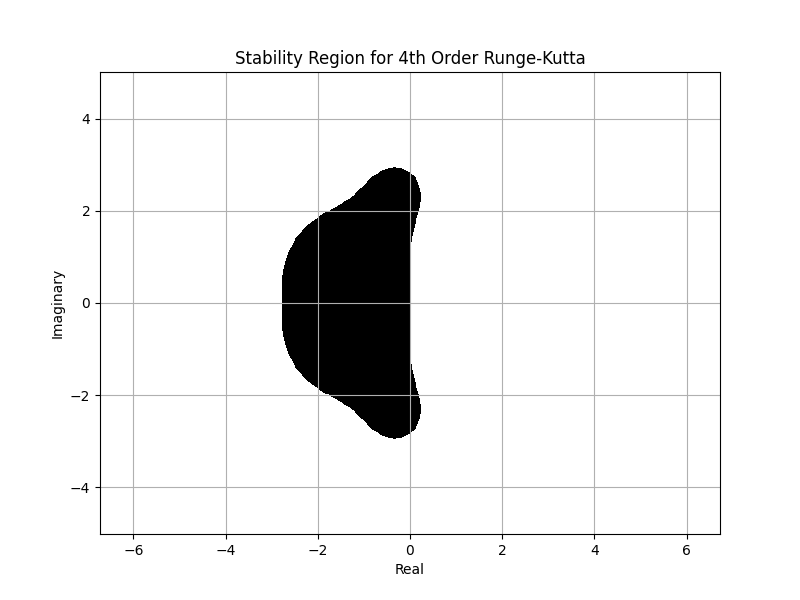
\includegraphics[width=0.8\textwidth]{RK4_stability.png}
\caption{The absolute stability region for Runge-Kutta 4 stages method.}
\label{fig:runge-kutta stability}
\end{figure}
The Interval of absolute stability for Runge-Kutta 4 is $\bar{h} \in (-2.78, 0)$, so we have $h < |\frac{2.78}{\lambda}|$, where $\lambda$ is the largest modulus eigenvalue of A.
Using the SciPy library in Python to find the largest modulus eigenvalue of the scaled discrete Laplacian matrix, we found that for absolute stability it is necessary to have $h < 3.5464 * 10^{-5}$.


\subsection*{Solving the system}
The exercise requests to compute the solution for $t\in(0,0.1]$ using different methods, first with ODE45, then Crank-Nicolson and BDF3, computing the final error as the infinite norm of the solutions obtained compared with the accurate solution, which has been loaded as an external file in the python script. \\[12pt]

\begin{tabular}{|c|c|c|c|}
\hline
METHOD & NUMBER OF STEPS & ERROR & CPU TIME \\ \hline
rk45 & 2367 & $4.5314*10^{-5}$ & 4.761  \\ \hline
Crank-Nicolson & 100 & $3.7837*10^{-5}$ &  0.611  \\ \hline
Crank-Nicolson & 1000 & $1.3976*10^{-7}$ & 2.027  \\ \hline
Crank-Nicolson & 10000 & $1.3967*10^{-9}$ & 17.711  \\ \hline
BDF3 & 100 & $7.0720*10^{-7}$ & 0.357  \\ \hline
BDF3 & 1000 & $7.2624*10^{-10}$ & 1.133  \\ \hline
BDF3 & 10000 & $2.2578*10^{-12}$ & 11.345  \\ \hline
\hline
\end{tabular}

\section{Exercise 6}

Consider the Lotka-Volterra equations :
\begin{equation}
\begin{cases}
x'(t) = x(t)( \alpha - \beta y(t)) , \\
y'(t) = y(t)(\gamma x(t) - \delta) , \\
x(0) = x_0 , \\
y(0) = y_0 .
\end{cases}
\end{equation}

Solve the IVP using Runge-Kutta 4 stages method, with parameters $\alpha = 0.2 , \beta = 0.01 , \gamma = 0.004 , \delta = 0.07 $ using the initial conditions $x_0 = 19 , y_0 = 22 , t_0 = 0, T = 300$ and step size $h = 10^{-3}$.

% Include a figure (Make sure to include the actual file in your LaTeX project)
\begin{figure}[H]
\centering
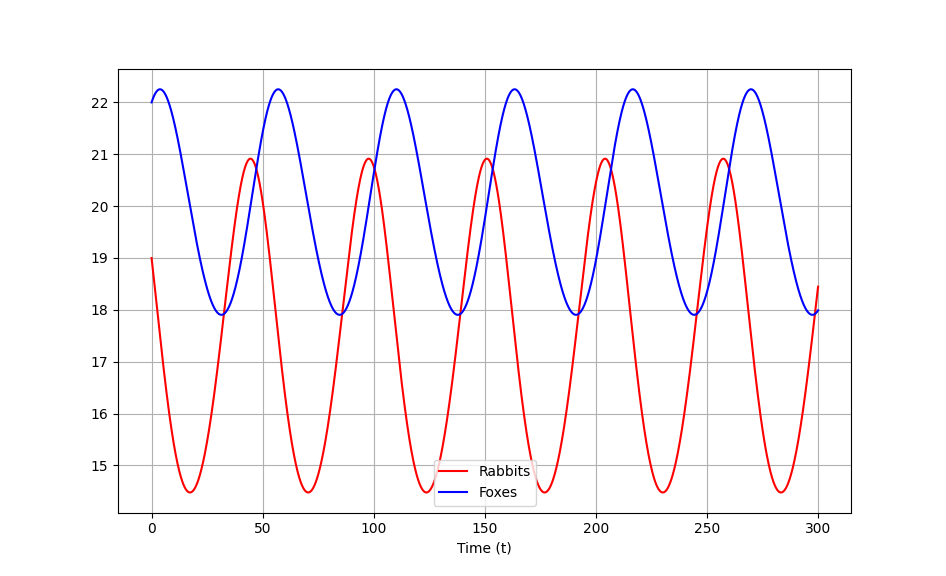
\includegraphics[width=0.8\textwidth]{lotka_volterra.png}
\caption{The numerical solution obtained by applying the Runge-Kutta 4 method to the Lotka-Volterra equations.}
\label{fig:lotka_volterra_solution}
\end{figure}


% Uncomment the following two lines if you have references
%\bibliography{your_bib_file}
%\bibliographystyle{ieeetr}

\end{document}
